% ============== Physik-Grundkurs Template (helles stählerndes Blau, XeLaTeX/LuaLaTeX) ==============
\documentclass[11pt,a4paper,oneside]{article}

% -------------------- Engine & Fonts --------------------
\usepackage{fontspec}
% Hauptschrift: sachlich, technisch (falls nicht installiert, fällt TeX auf Systemschrift zurück)
%\setmainfont{Fira Sans}[Scale=MatchLowercase]
%\setsansfont{Fira Sans}
\usepackage{unicode-math}
\setmathfont{Libertinus Math}

% -------------------- Pakete --------------------
%% --- Sprachen und Kodierung ---
\usepackage[ngerman]{babel}   % deutsche Sprachunterstützung
\usepackage{csquotes}         % korrekte Anführungszeichen

% --- Mathematik ---
\usepackage{amsmath}          % grundlegende Mathematikumgebung
\usepackage{mathtools}        % Erweiterungen für amsmath
\usepackage{physics}          % nützliche Makros für Physik
\usepackage{dsfont}           % Mengensymbole (z. B. \mathds{R})

% --- Schriften ---
% für XeLaTeX/LuaLaTeX: fontspec, unicode-math und Libertinus
\usepackage{fontspec}
\usepackage{unicode-math}
\setmainfont{Libertinus Serif}
\setsansfont{Libertinus Sans}
\setmonofont{Libertinus Mono}
\setmathfont{Libertinus Math}

% --- Layout und Typografie ---
\usepackage[top=3cm, bottom=3cm, left=2.5cm, right=2.5cm]{geometry}
\usepackage{microtype}        % schönerer Randausgleich
\usepackage[onehalfspacing]{setspace} % 1,5-facher Zeilenabstand
\usepackage{tocloft}          % Inhaltsverzeichnis anpassen
\renewcommand{\cftsecleader}{\cftdotfill{\cftdotsep}} 

% --- Farben und Boxen ---
\usepackage{xcolor}
\newcommand{\ricardo}[1]{%
	\colorbox{ForestGreen}{\color{white}\textsf{\textbf{Ricardo}}}%
	\textcolor{ForestGreen}{#1}%
}

% --- Tabellen und Listen ---
\usepackage{tabularx}
\usepackage{longtable}
\usepackage{dcolumn}
\usepackage{adjustbox}

% --- Grafiken ---
\usepackage{graphicx}
\usepackage{here}
\usepackage{floatflt}     % Bilder im Fließtext (eher alt)
\usepackage{epsfig}       % alte EPS-Unterstützung
\usepackage{epstopdf}     % Konvertierung EPS -> PDF

% --- Zitate und Literatur ---
\usepackage{cite}
\usepackage{bibgerm}      % deutsche BibTeX-Stile (alt; besser biblatex)

% --- Sonstiges ---
\usepackage{acro}         % Abkürzungsverzeichnis
\usepackage{blindtext}
\usepackage{lipsum}
\usepackage{listings}     % Quellcode
\usepackage{lettrine}     % Initialen
\usepackage[cute inductors,siunitx]{circuitikz} % Schaltpläne

\usepackage{amsmath}
\usepackage[ngerman]{babel}
\usepackage{acro}
\usepackage{microtype}
\usepackage{geometry}
\usepackage{titlesec}
\usepackage{fancyhdr}
\usepackage{xcolor}
\usepackage{pagecolor}
\usepackage[most]{tcolorbox}
\tcbuselibrary{skins,breakable,theorems}
\usepackage{enumitem}
\usepackage{caption}
\usepackage{everypage}
\usepackage{graphicx}
\usepackage{float}
\usepackage{wrapfig}
\usepackage{caption}
\usepackage{booktabs} % schöne Tabellenkanten
% -------------------- Tikz --------------------
\usepackage{tikz}
\usetikzlibrary{decorations.pathreplacing} % für geschweifte Klammern
\usetikzlibrary{shadings,shadows,calc}
\usetikzlibrary{arrows.meta,decorations.markings}

% --------------------PGF Plots ---------------------




% -------------------- Layout --------------------
\geometry{
	left=28mm, right=28mm, top=28mm, bottom=28mm,
	marginparwidth=36mm, marginparsep=6mm
}

% -------------------- Farben (helles stählerndes Blau, dezenter Verlauf) --------------------
\definecolor{PageBGTop}{RGB}{225,233,241}   % sehr helles Stahlblau oben
\definecolor{PageBGBot}{RGB}{245,250,255}   % fast weiß-blau unten
\definecolor{BodyText}{RGB}{28,38,48}       % dunkles Schiefergrau für Text
\definecolor{AccentSteel}{RGB}{100,149,237} % steel/cornflower blue Akzent
\definecolor{AccentSky}{RGB}{150,200,255}   % helleres Blau
\definecolor{AccentWarn}{RGB}{255,120,55}   % Warnorange
\definecolor{BoxInner}{RGB}{250,253,255}    % fast weiß für Boxmitte
\definecolor{MarginalGray}{RGB}{120,130,140}

\definecolor{AccentBlue1}{RGB}{200,220,255}   % sehr helles Blau
\definecolor{AccentBlue2}{RGB}{140,170,230}   % mittelhell
\definecolor{AccentBlue3}{RGB}{80,120,200}    % dunkleres Blau
\definecolor{AccentBlue4}{RGB}{40,70,130}     % sehr dunkel
\definecolor{AccentBlack}{RGB}{25,25,35}      % fast schwarz

\definecolor{TextCream}{RGB}{250,250,245}     % helle Schrift
\definecolor{TextDark}{RGB}{30,30,40}         % dunkle Schrift
\definecolor{BoxBackground}{RGB}{255,255,255}% farblos/weiß

\definecolor{AccentSteelDark}{RGB}{50,90,160}   % dunkles Stahlblau für Section
\definecolor{AccentSteel}{RGB}{80,130,220}     % mittleres Blau für Subsection
\definecolor{AccentSky}{RGB}{150,200,255}      % helles Blau für Subsubsection



% Setze Seitenhintergrund mit TikZ-Gradient (funktioniert mit Xe/LuaLaTeX)
\pagecolor{white} % temporär; wir zeichnen Gradient mit TikZ auf jeder Seite
\AddEverypageHook{%
	\begin{tikzpicture}[remember picture,overlay]
		\shade[left color=PageBGTop,right color=PageBGBot] (current page.north west) rectangle (current page.south east);
	\end{tikzpicture}
}

% Textfarbe
\color{BodyText}

% -------------------- Kopf / Fuß --------------------
\pagestyle{fancy}
\fancyhf{}
\renewcommand{\headrulewidth}{0pt}
\setlength{\headheight}{18pt}
%\fancyhead[L]{\sffamily\small Grundkurs Physik\quad -- \quad Skript}
\fancyfoot[C]{\scriptsize\sffamily Ferdinand-Braun Schule \quad • \quad Grundkurs Physik \quad • \quad \thepage}
\fancyfoot[R]{\begin{tikzpicture}[remember picture,overlay]
		\draw[line width=0.8pt,color=AccentSteel!60!black] ($(current page.south west)+(28mm,20mm)$) -- ($(current page.south east)+(-28mm,20mm)$);
\end{tikzpicture}}

% -------------------- Titel-Styles (harmonischer Blauverlauf) --------------------
\titleformat{\section}{\normalfont\large\bfseries\sffamily\color{AccentSteelDark}}{\thesection}{1em}{}
\titleformat{\subsection}{\normalfont\normalsize\bfseries\sffamily\color{AccentSteel}}{\thesubsection}{0.8em}{}
\titleformat{\subsubsection}{\normalfont\normalsize\bfseries\sffamily\color{AccentSky}}{\thesubsubsection}{0.6em}{}


% ========================= TCBOX BASIS-STIL (physikalische, helle Boxen mit Verlauf) =========================
\tcbset{
	mybase/.style={
		enhanced,
		breakable,
		boxrule=0.9pt,
		colframe=black!20,
		colback=BoxBackground,      % Hintergrund farblos
		colupper=TextDark,
		arc=1mm,
		boxsep=5pt,
		left=15pt,right=15pt,top=15pt,bottom=15pt,
		before skip=8pt, after skip=8pt,
		attach boxed title to top left={yshift=-0.25mm-\tcboxedtitleheight/2, xshift=10mm},
		boxed title style={
			arc=3mm,
			left=6pt,right=6pt,top=3pt,bottom=3pt,
			boxrule=0pt
		},
		fonttitle=\sffamily\bfseries\small,
		title after break=\vspace{4pt}
	}
}

% -------------------- THEOREM (theo) --------------------
\newtcolorbox[auto counter,number within=section]{theo}[2][]{%
	mybase,
	colframe = AccentBlue1!80!black,
	colbacktitle = AccentBlue1!95!black,
	coltitle = TextDark,
	title = {Theorem~\thetcbcounter: #2},
	#1
}

% -------------------- BEISPIEL (exem) --------------------
\newtcolorbox[auto counter,number within=section]{exem}[2][]{%
	mybase,
	colframe = AccentBlue2!80!black,
	colbacktitle = AccentBlue2!95!black,
	coltitle = TextCream,
	title = {Beispiel~\thetcbcounter: #2},
	#1
}

% -------------------- AUFGABE (aufgabe) --------------------
\newtcolorbox[auto counter,number within=section]{aufgabe}[2][]{%
	mybase,
	colframe = AccentBlue3!80!black,
	colbacktitle = AccentBlue3!95!black,
	coltitle = TextCream,
	title = {Aufgabe~\thetcbcounter: #2},
	#1
}

% -------------------- LÖSUNG (loesung) --------------------
\newtcolorbox[use counter from=aufgabe]{loesung}[2][]{%
	mybase,
	colframe = AccentBlue4!85!black,
	colbacktitle = AccentBlue4!95!black,
	coltitle = TextCream,
	title = {Lösung~\thetcbcounter: #2},
	#1
}

% -------------------- Hinweis-Box --------------------
\newtcolorbox{infobox}[1][]{%
	mybase,
	colframe = AccentBlack!80!black,
	colbacktitle = AccentBlack,
	coltitle = TextCream,
	title = {Hinweis},
	#1
}

% -------------------- Experiment-Box --------------------
\newtcolorbox[auto counter,number within=section]{experiment}[2][]{%
	mybase,
	colframe = AccentBlue2!80!black,
	colbacktitle = AccentBlue2!95!black,
	coltitle = TextCream,
	title = {Experiment~\thetcbcounter: #2},
	#1
}

% ==================== Datum Makro ====================
\newcommand{\lessondate}[1]{\noindent\hfill\textcolor{MarginalGray}{\textsc{#1}} \\ \vspace{0.5cm}}

% ==================== Feines Titelblatt ====================
\newcommand{\MakeArtTitle}[4]{%
	\begin{titlepage}
		\begin{tikzpicture}[remember picture,overlay]
			\shade[left color=PageBGTop,right color=PageBGBot] (current page.north west) rectangle (current page.south east);
		\end{tikzpicture}
		\vspace*{25mm}
		\begin{center}
			{\Huge\sffamily\bfseries\color{AccentSteel} #1 \par}
			\vspace{8mm}
			{\Large\itshape\color{AccentSky} #2 \par}
			\vspace{12mm}
			{\Large\scshape\color{BodyText} #3 \par}
			\vspace{6mm}
			{\small\color{MarginalGray} #4 \par}
			\vspace{90mm}
			
\includegraphics[width=0.75\textwidth]{image.png} % Logo: Pfad anpassen
		\end{center}
	\end{titlepage}
}

% ==================== Dokumentbeginn ====================
\begin{document}
	
	% Titelblatt
	\MakeArtTitle{Grundkurs Physik Q3 Hessen}{Skript und Übungsaufgaben}{Shamsher Singh Kalsi}{Berufliches Gymnasium — Ferdinand-Braun Schule \\ Kursleiter: Herr Dr. Frank Diegmüller}
	
	\tableofcontents
	\bigskip
	\clearpage
	
	\section{Einleitung}
	\lessondate{19.08.2025}\\
	Dieses Skript ist als leicht lesbare Sammlung von Vorlesungsnotizen, Experimentbeschreibungen und Übungsaufgaben für den Physik-Grundkurs gedacht. Es wurde die alte Duden Paetek Formel abgelöst und von dem IQB eine Einheitliche veröffentlicht. Auf moodle steht die neue Formelsammlung. Thomsoneschwingungsgleichung. 
	
	\subsection{Nachschlaginhalte}
	
	\subsubsection{SI-Vorsätze}
	\lessondate{02.09.2025}\\
	\begin{table}[ht]
		\centering
		\caption{SI-Vorsätze (Symbole und Faktoren)}
		\label{tab:si-prefixes}
		\begin{tabular}{@{} l c c @{}}
			\toprule
			Name & Symbol & Faktor \\
			\midrule
			quetta  & Q  & \(10^{30}\) \\
			ronna   & R  & \(10^{27}\) \\
			yotta   & Y  & \(10^{24}\) \\
			zetta   & Z  & \(10^{21}\) \\
			exa     & E  & \(10^{18}\) \\
			peta    & P  & \(10^{15}\) \\
			tera    & T  & \(10^{12}\) \\
			giga    & G  & \(10^{9}\)  \\
			mega    & M  & \(10^{6}\)  \\
			kilo    & k  & \(10^{3}\)  \\
			hecto   & h  & \(10^{2}\)  \\
			deca    & da & \(10^{1}\)  \\
			(kein Vorsatz) &  & \(10^{0}\)  \\
			deci    & d  & \(10^{-1}\) \\
			centi   & c  & \(10^{-2}\) \\
			milli   & m  & \(10^{-3}\) \\
			micro   & \(\mu\) & \(10^{-6}\) \\
			nano    & n  & \(10^{-9}\) \\
			pico    & p  & \(10^{-12}\) \\
			femto   & f  & \(10^{-15}\) \\
			atto    & a  & \(10^{-18}\) \\
			zepto   & z  & \(10^{-21}\) \\
			yocto   & y  & \(10^{-24}\) \\
			ronto   & r  & \(10^{-27}\) \\
			quecto  & q  & \(10^{-30}\) \\
			\bottomrule
		\end{tabular}
	\end{table}
	
	
	
	\newpage
	
	\lessondate{17.09.2025}\\
	\subsection*{Regularieren für die Arbeit}
	\begin{itemize}
		\item Ergebnisse haben immer eine EInheit - sonst keine Bewertung 
		\item Die Struktur der Aufgabenstellung muss eingehalten werden 
		\item Endergebnisse doppelt unterstreichen oder Antwortsatz 
		\item Ergebnisse werden immer auf zwei nachkommastellen gerundet 
		\item Alle Formeln in der Formelsammlung als gegeben anzusehen 
		\item Lösungsweg ordentlich dokumentieren 
		\item SI-Vorsätze wenn nötig bei den Ergebnissen nennen
		\subsection*{Wie rechne ich eine Aufgabe}
		\begin{itemize}
			\item Formel aus der Formelsammlung suchen 
			\item Formel nach der gesuchten Größe umstellen 
			\item Zahlenwerte einsetzen - keine Naturkonstanten - lieber vom Taschenrechner nehmen (Shift + 7)
			\item Mit dem Taschenrechner ausrechnen 
			\item Ergebnis präsentieren 
		\end{itemize}
	\end{itemize}
	
	
	
	\newpage
	
	\section{Wiederholung}
	%\lessondate{19.08.2025}\\
	
	\subsection{Herleitung der Interferenz und Beugung am Doppelspalt}
	%\lessondate{19.08.2025}\\
	Die Überlagerung von Lichtwellen am Doppelspalt ist eines der klassischen Experimente der Wellenoptik und wurde erstmals von \textsc{Thomas Young} im Jahr 1801 durchgeführt. Es zeigt, dass Licht Welleneigenschaften besitzt, da sich charakteristische Interferenzmuster nur durch das Prinzip der Überlagerung erklären lassen. Die beobachteten Helligkeitsmaxima und -minima entstehen durch konstruktive und destruktive Interferenz zweier kohärenter Wellenzüge, die durch die beiden Spalte hindurchlaufen.
	
	
	\begin{minipage}[t]{0.45\textwidth}
		\vspace{0mm}
		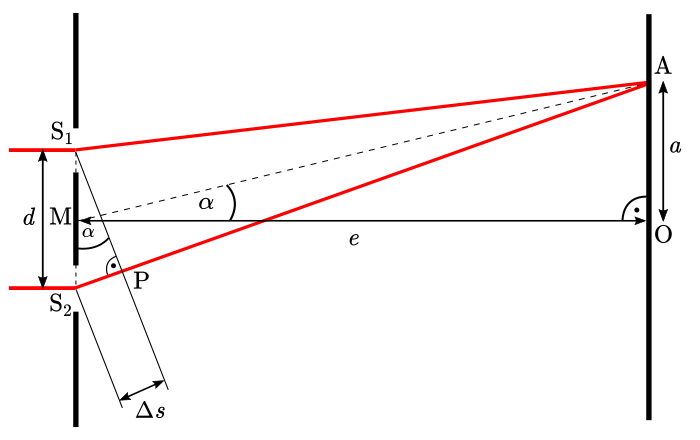
\includegraphics[width=\textwidth]{Doppelspalt_Einstiegsaufgaben_Bild.png}
		\captionof{figure}{Doppelspalt Nahaufnahme}
	\end{minipage}%
	\hfill
	\begin{minipage}[t]{0.45\textwidth}
		\vspace{0pt} % zwingt die Oberkante wirklich nach oben
		\begin{itemize}
			\item [$d:$] Abstand der Mittelpunkte der Spalten 
			\item [$e:$] Abstand zwischen Doppelspalt und Schirm 
			\item [$a:$] Abstand eines Punktes $A$ auf dem Schirm zum Punkt $O$ , an dem sich das 0. Maximum befindet
			\item [$\alpha:$] Weite des Winkels 
		\end{itemize}
	\end{minipage}

	Die Bedingung für konstruktive Interferenz lautet
	\begin{align*}
		\sin \alpha &= \frac{k \cdot \lambda}{d}, \quad k \in \mathbb{Z},
	\end{align*}
	wobei $k$ die Ordnung des Maximums bezeichnet. Für destruktive Interferenz ergibt sich entsprechend
	\begin{align*}
		\sin \alpha &= \frac{(2k - 1)\cdot \frac{\lambda}{2}}{d}, \quad k \in \mathbb{N}.
	\end{align*}
	
	Für kleine Winkel $\alpha$ kann man näherungsweise $\sin \alpha \approx \tan \alpha \approx \frac{a}{e}$ setzen, sodass die Position $a$ der Maxima auf dem Schirm berechnet werden kann:
	\begin{align*}
		a_k \approx \frac{e \cdot k \cdot \lambda}{d}.
	\end{align*}
	
	
	\subsection*{Wichtige Wellenphänomene (vgl. Tipler, S. 493)}
	
	\begin{theo}{Definitionen grundlegender Wellenphänomene}
		\begin{enumerate}
			\item \textbf{Reflexion:} Richtungsänderung einer Welle an einer Grenzfläche, sodass sie in das Ursprungsmedium zurückkehrt (z.~B. Spiegel).
			\item \textbf{Beugung:} Ablenkung und Ausbreitung einer Welle hinter Hindernissen oder Öffnungen, die mit der Wellenlänge vergleichbar sind.
			\item \textbf{Brechung:} Änderung der Ausbreitungsrichtung einer Welle beim Übergang in ein Medium mit unterschiedlicher Ausbreitungsgeschwindigkeit.
		\end{enumerate}
	\end{theo}
	
	%\begin{figure}[h]
	%	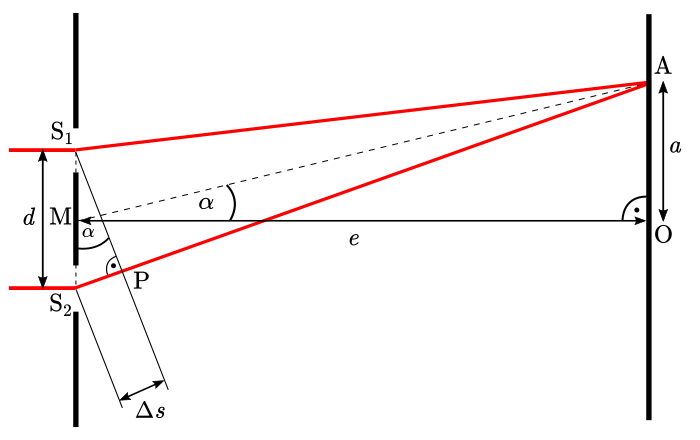
\includegraphics[width=0.5\textwidth]{Doppelspalt_Einstiegsaufgaben_Bild.png}
	%\end{figure}
	
	%\newpage
	
	%\lessondate{02.09.2025}\\
	%\subsection{Lösung A.2}
	
	
	
	
	\newpage
	\lessondate{02.09.2025}\\
	
	\begin{aufgabe}{Bohr'sches Atommodell}
		\small
		\begin{itemize}[left=20mm]
			\item [\textbf{Aufgabe 1}] Leitet aus den beiden Gleichungen 
			\begin{align*}
				2 \cdot \pi \cdot r &= n \cdot \lambda \\
				\lambda &= \frac{h}{mv}
			\end{align*}
			die Quantenbedingung her. Dazu wird eine Gleichung nach der Wellenlänge aufgelöst und in die
			andere eingesetzt. Die Wellenlänge ist somit eliminiert. In Gleichung 1 kann man erkennen, dass man
			dem Kreisumfang eine De-Broglie-Welle einbeschreibt. Wir werden diese Gleichungen noch später in
			Unterricht besprechen.
			\item [\textbf{Aufgabe 2}] 
			Das Elektron hat die Masse m und die negative Elementarladung e. Es bewegt sich mit der Bahngeschwindigkeit v auf einer Kreisbahn mit dem Radius r um den Atomkern.
			\begin{itemize}[left=-10mm]
				\item [A:] Erstelle eine Skizze des Wasserstoffatoms mit allen notwendigen und sinnvollen Angaben. Zeichne dabei mehrere Elektronenschalen ein.
				\item [B:] Gebe die Formel zur Bestimmung der Zentrifugalkraft an, die auf das Elektron wirkt. Diese
				Kraft wirkt nach außen.
				\item [C:] Welche Gegenkraft wirkt auf das Elektron, damit es auf der Kreisbahn bleibt? Diese Gegenkraft muss zum Atomkern hin gerichtet sein, es stellt somit die Zentripetalkraft dar. Benenne diese Gegenkraft.
				\item [D:] Gebe nun diese Formel aus b) zur Bestimmung der Gegenkraft an. \\
				Diese beiden Gleichungen sind bereits im Rutherfordschen Atommodell gültig. Jetzt kommt noch die
				Quantenbedingung hinzu. Jetzt wird die Quantenbedingung aus Aufgabe 1 benötigt.
				\item [E:]  Gebe mit Hilfe dieser drei Gleichungen eine Formel zur Bestimmung des Radius $r$ der Elektronenbahn in Abhängigkeit der Elektronenmasse und Elektronenladung, der Quantenzahl und
				evtl. Naturkonstanten an, also $r_n = f(n)$
				\item [F:] Bestimme den Radius der innersten Elektronenbahn zahlenmäßig.
				\item [G:] Bestimme alle weiteren Radien in Abhängigkeit vom Radius der innersten Bahn $r_1$
				\item [H:] estimme mit Hilfe dieser drei Gleichungen die Geschwindigkeit der Elektronen in Abhängigkeit der Elektronenladung, der Quantenzahl und evtl. Naturkonstanten formelmäßig, also $v_n = f(n)$
				\item [I:] Bestimme die Geschwindigkeit der Elektronen auf der innersten Bahn zahlenmäßig.
				\item [J:] Bestimme alle weiteren Geschwindigkeiten in Abhängigkeit der Geschwindigkeit auf der innersten Bahn.
			    \item [K:] Auf welcher Bahn hat das Elektron die größtmögliche Geschwindigkeit? Gebe diese Geschwindigkeit als Faktor der Lichtgeschwindigkeit an!
				\item [L:] Bestimme die kinetische Energie der Elektronen in Abhängigkeit der Elektronenmasse und -
				ladung, der Quantenzahl und evtl. Naturkonstanten formelmäßig, also $E_{kin} = f(n)$
				
				\newpage
				
				\item [M:] Was ist die potentielle Energie, wenn es um Ladungen in einem elektrischen Feld geht? Hinweis:
				siehe BG12.1. Siehe auch Aufgabenteil b).
				\item [N:] Bestimme die potentielle Energie der Elektronen in Abhängigkeit der Elektronenmasse und Elektronenladung, der Quantenzahl und evtl. Naturkonstanten formelmäßig, also $E_{pot} = f(n)$
				\item [O:] Vergleichen Sie $E_{kin}$ mit $E_{pot}$
				\item [P:] Bestimmen Sie $E_{ges} = E_{kin} + E_{pot}$ 
				\item [Q:] Bestimme die Gesamtenergie $E_n$ der Elektronen auf der n-ten Quantenbahn in Abhängigkeit der
				Elektronenmasse und -ladung, der Quantenzahl und evtl. Naturkonstanten formelmäßig, also $E_ges = f(n)$. Nutzen Sie hierbei unbedingt die Einheit Elektronenvolt!
				\item [R:] telle diese Formel in einem Grafen (Energieniveauschema) dar. Y-Achse: Energie $E_n$. Schaue in
				der Literatur nach.		
			\end{itemize}
		\end{itemize}
	\end{aufgabe}
	
	
	
	\newpage
	
	
	\subsection{Probleme des Atommodells von Rutherford}
	
	Das Rutherford-Modell kann die Stabilität der Atome nicht erklären. 
	Nach klassischer Elektrodynamik beschreibt ein Elektron auf Kreisbahn 
	eine beschleunigte Bewegung. Beschleunigte Ladungen strahlen jedoch 
	elektromagnetische Energie ab und müssten Energie verlieren – 
	das Elektron stürzte in den Kern, stabile Atome wären unmöglich. \\
	
	Ebenso erklärt das Modell nicht die quantisierte Emission und Absorption 
	von Licht. Experimente wie die Balmer-Serie, die Umkehr der Natrium-D-Linie 
	oder der Franck-Hertz-Versuch zeigen eindeutig, dass Atome nur diskrete 
	Energien aufnehmen oder abgeben können. Im Rutherford-Modell dagegen 
	sind alle Bahnradii und Elektronengeschwindigkeiten erlaubt, 
	die Gesamtenergie der Elektronen wäre beliebig.
	
	\begin{theo}{Bohrs Lösung durch drei Postulate (1913)}
		Bohr übertrug die Quantenvorstellungen von Planck und Einstein 
		auf den Atomaufbau und stellte drei Postulate auf, 
		die zunächst vor allem beim Wasserstoff erfolgreich waren. 
		Das dritte Postulat ist aus heutiger Sicht überholt.
		
		\begin{enumerate}
			\item \textbf{Energiequantelung:} 
			Ein Elektron im Atom kann nur diskrete Energiewerte $E_n$ besitzen.
			
			\item \textbf{Strahlung:} 
			Die Frequenz $f$ der Strahlung ergibt sich aus der Energiedifferenz:
			\[
			h f = E_m - E_n \quad (m > n, \; m,n \in \mathbb{N})
			\]
			
			\item \textbf{Bahnen (Quantenbedingung):} 
			Elektronen bewegen sich nur auf stationären Bahnen ohne Energieabstrahlung. 
			Es gilt:
			\[
			m_e r_n v_n = \frac{n h}{2 \pi}
			\]
		\end{enumerate}
	\end{theo}
	
	\begin{loesung}{Bohr'sches Atommodell}
		\subsection*{Aufgabe 1}		
		Setzt man $\lambda = \tfrac{h}{mv}$ in $2 \pi r = n \lambda$ ein, so folgt:
		\begin{align*}
			2 \pi r &= n \cdot \frac{h}{m v} \\
			m v r &= \frac{n h}{2 \pi}.
		\end{align*}
		
		Damit erhält man die Quantenbedingung für den Bahndrehimpuls:
		\[
		L = m v r = n \hbar \quad \text{mit} \quad \hbar = \frac{h}{2 \pi}.
		\]
	\end{loesung}
	
	
	
	\begin{loesung}{Bohr'sches Atommodell}
		\subsection*{Aufgabe 2 A bis D - Tipler Seite 1231}
		\vspace{5mm}
		\begin{minipage}[t]{0.5\textwidth}
			\begin{tikzpicture}[scale=1.25]
				
				% Atomkern
				\shade[ball color=red!50] (0,0) circle (0.3) node[white] {p$^+$};
				
				% Erste Elektronenschale
				\draw[thick] (0,0) circle (1);
				% Elektron auf erster Schale
				\shade[ball color=blue!50] (1,0) circle (0.15) node[right=2pt] {e$^-$};
				
				% Zweite Elektronenschale
				\draw[thick,dashed] (0,0) circle (1.8);
				% Elektronen auf zweiter Schale
				\shade[ball color=blue!50] (1.8,0) circle (0.12);
				\shade[ball color=blue!50] (-1.8,0) circle (0.12);
				
				% Radius r beschriften (zum Elektron auf erster Schale)
				\draw[<->] (0,0) -- (0.7,0.7)
				node[midway,above left] {$r$};
				
				% Geschwindigkeitspfeil (Tangentialrichtung)
				\draw[-{Latex[length=3mm]}] (1,0) -- (1,0.8)
				node[right] {$v$};
				
				% Zentripetalkraft (zum Kern hin)
				\draw[-{Latex[length=3mm]},red,thick] (1,0) -- (0.2,0)
				node[midway,below] {$F_\text{z}$};
				
			\end{tikzpicture}
		\end{minipage}
		\hfill
		\begin{minipage}[t]{0.5\textwidth}
			\vspace{-40mm}
			\begin{itemize}
				\item[B:] \textbf{Zentrifugalkraft:}\\
				$
				F_\text{zentrifugal} = \frac{m v^2}{r}
				$
				\item[C:] \textbf{Gegenkraft:} Coulomb-Kraft zwischen Elektron und Kern
				\item[D:] \textbf{Zentripetalkraft:} 
				\[
				F_\text{Coulomb} = \frac{1}{4\pi \varepsilon_0} \cdot \frac{Z e^2}{r^2} 
				\]
				\[
				F_C = \frac{1}{4 \cdot \pi \cdot \varepsilon_0 \cdot \varepsilon_r} \cdot \frac{Q_1 \cdot Q_2}{r^2}
				\]
			\end{itemize}
		\end{minipage}
		
		\vspace{5mm}
		\begin{infobox}
			\small
			Stabilität liegt vor, weil gilt 
			\[
			F_\text{zentrifugal} = F_\text{Coulomb}.
			\]
			\footnote{(Vgl. Tipler, Abb. 34.3 und Gl. (34.5))}
		\end{infobox}
	\end{loesung}
	
	\lessondate{04.09.2025}\\
	\vspace{-1cm}
	\begin{loesung}{Bohr'sches Atommodell}
		\subsection*{Aufgabe E}
		\[
		\boxed{
		F_\text{coulomb} = \frac{1}{4 \pi \epsilon_0} \cdot \frac{Ze^2}{r^2}, \qquad
		F_\text{zentrifugal} = \frac{mv^2}{r}, \qquad m\cdot v \cdot r = n \cdot \hbar 
		}
		\]
		\begin{align*}
			F_\text{coulomb} &= F_\text{zentrifugal} \\\\
			\frac{1}{4 \cdot \pi \cdot \varepsilon_0} \cdot \frac{Ze^2}{r^2} &= \frac{m \cdot v^2}{r}, \quad v = \frac{n \cdot \hbar}{m \cdot r}\\\\
			\frac{1}{4 \cdot \pi \cdot \varepsilon_0} \cdot \frac{Ze^2}{r^2} &=  \frac{m \cdot \left( \frac{n \cdot \hbar}{m \cdot r}\right)^2 }{r}
		\end{align*}
	\end{loesung}
	
	\newpage
	
	\begin{loesung}{Bohr'sches Atommodell}
		\subsection*{Aufgabe E}
		\begin{align*}
			\frac{1}{4 \cdot \pi \cdot \varepsilon_0} \cdot \frac{Ze^2}{r^2} &= m \cdot \frac{n^2 \cdot \hbar^2}{m^2 \cdot r^2} \cdot \frac{1}{r} \quad | \cdot r^3 \\\\
			\frac{1}{4 \cdot \pi \cdot \varepsilon_0} \cdot Ze^2 \cdot r&= \frac{n^2 \cdot \hbar^2}{m}\\\\
			r &= \boxed{ \frac{4 \cdot \pi \cdot \varepsilon_0 \cdot \hbar^2}{m \cdot e^2} \cdot \frac{n^2}{Z}}
		\end{align*}
		
		\subsection*{Aufgabe F}
		\begin{align*}
			r &= \frac{4 \cdot \pi \cdot \varepsilon_0 \cdot \hbar^2}{m \cdot e^2} \cdot \frac{n^2}{Z}, \qquad
			r_1 = \frac{4 \cdot \pi \cdot \varepsilon_0 \cdot \hbar^2}{m \cdot e^2} \cdot \underbrace{\frac{(1)^2}{(1)}}_{1}\\\\
			r_1 &\approx \boxed{5.29 \cdot 10^{-11}m = 52.9 pm}
		\end{align*}
		\subsection*{Aufgabe G}
		\begin{align*}
			r_n &= r_1 \cdot \frac{n^2}{Z}\\ \quad
			r_2 &= r_1 \cdot \frac{(2)^2}{1} = 5.29 \cdot 10^{-11}m \cdot 4 = \boxed{21.16 \cdot 10^{-11}m}\\
			r_3 &= r_1 \cdot \frac{(3)^2}{1} = 5.29 \cdot 10^{-11}m \cdot 9 = \boxed{47.61 \cdot 10^{-11}m}
		\end{align*}
	\end{loesung}

	\footnote{
	\begin{align*}
		\varepsilon_0 &\approx 8.854 \cdot 10^{-12} \frac{F}{m} \quad && \text{Permittivität des Vakuums} \\
    	\hbar &= 1.054 \cdot 10^{-34} \, \text{Js} && \text{reduziertes plancksches Wirkungsquantum} \\
		m_e &= 9.109 \cdot 10^{-31} \, \text{kg} && \text{Masse des Elektrons} \\
		e &= 1.602 \cdot 10^{-19} \, \text{C} && \text{Elementarladung}
	\end{align*}
	}
	
	\newpage
	
	\begin{loesung}{Bohr'sches Atommodell}
		\subsection*{Aufgabe H}
		\[
		F_\text{coulomb} = \frac{1}{4 \pi \epsilon_0} \cdot \frac{Ze^2}{r^2}, \qquad
		F_\text{zentrifugal} = \frac{mv^2}{r}, \qquad m\cdot v \cdot r = n \cdot \hbar 
		\]
		\begin{align*}
			F_\text{coulomb} &= F_\text{zentrifugal} \\\\
			\frac{1}{4 \pi \varepsilon_0} \cdot \frac{Ze^2}{r^2} &= \frac{m v^2}{r}, \qquad r = \frac{n \hbar}{m v} \\\\
			\frac{1}{4 \pi \varepsilon_0} \cdot \frac{Ze^2}{\left(\tfrac{n \hbar}{m v}\right)^2} &= \frac{m v^2}{\tfrac{n \hbar}{m v}} \\\\
			\frac{1}{4 \pi \varepsilon_0} \cdot Ze^2 \cdot \frac{m^2 v^2}{n^2 \hbar^2} &= \frac{m^2 v^3}{n \hbar} \quad | : (m^2 v) \\\\
			\frac{1}{4 \pi \varepsilon_0} \cdot Ze^2 \cdot \frac{1}{n^2 \hbar^2} &= \frac{v}{n \hbar} \\\\
			%v &= \boxed{\frac{Ze^2}{4 \pi \varepsilon_0 \hbar} \cdot \frac{1}{n}}
		\end{align*}
		\vspace{-10mm}
		\[
		\boxed{v = \frac{Ze^2}{4 \pi \varepsilon_0 \hbar} \cdot \frac{1}{n}}
		\]
	\end{loesung}
	
	\lessondate{10.09.2025}\\
	\vspace{-15mm}
	\begin{loesung}{Bohr'sches Atommodell}
		\subsection*{Aufgabe I}
			Wir verwenden die bereits hergeleitete Formel
		\[
		v = \frac{Z e^2}{4\pi\varepsilon_0\hbar}\cdot\frac{1}{n}.
		\]
		Für das Wasserstoffatom mit \(Z=1\) und auf der innersten Bahn \(n=1\) gilt somit
		\[
		v_1 = \frac{e^2}{4\pi\varepsilon_0\hbar}.
		\]
		Numerisch ergibt das (mit den in den Fußnoten angegebenen Konstanten)
		\[
		\boxed{v_1 \approx 2{,}187691\times 10^{6}\ \mathrm{m/s}.}
		\]
	\end{loesung}
	
	\begin{loesung}{Bohr'sches Atommodell}
		\subsection*{Aufgabe J}
		Da \(v\propto 1/n\) folgt für beliebige Bahnen
		\[
		\boxed{v_n = \frac{v_1}{n} = \frac{Z e^2}{4\pi\varepsilon_0\hbar}\cdot\frac{1}{n}.}
		\]
		Damit sind die Geschwindigkeiten der höheren Bahnen einfach um den Faktor \(1/n\) gegenüber der innersten Bahn reduziert.\\
		\subsection*{Aufgabe K}
		Die Geschwindigkeit \(v_n\) fällt mit zunehmender Quantenzahl \(n\), da sie umgekehrt von \(n\) abhängt. Daher ist die größtmögliche Geschwindigkeit die auf der kleinsten erlaubten Bahn \(n=1\):
		\[
		v_\text{max} = v_1.
		\]
		Man kann \(v_\text{max}\) als Bruch der Lichtgeschwindigkeit \(c\) angeben:
		\[
		\boxed{\frac{v_\text{max}}{c} \approx 0{,}0073}
		\]
		\subsection*{Aufgabe L}
		\begin{align*}
			E_\text{kin} &= \frac{1}{2} m v^2, \qquad
			v = \frac{Z e^2}{4 \pi \varepsilon_0 \hbar} \cdot \frac{1}{n} \\\\
			E_\text{kin} &= \frac{1}{2} m \left(\frac{Z e^2}{4 \pi \varepsilon_0 \hbar} \cdot \frac{1}{n}\right)^2 = \frac{1}{2} m \frac{Z^2 e^4}{16 \pi^2 \varepsilon_0^2 \hbar^2} \cdot \frac{1}{n^2} \\\\
			&= \frac{m Z^2 e^4}{32 \pi^2 \varepsilon_0^2 \hbar^2} \cdot \frac{1}{n^2}
		\end{align*}
		\[
		\boxed{E_\text{kin}(n) = \frac{m Z^2 e^4}{32 \pi^2 \varepsilon_0^2 \hbar^2} \cdot \frac{1}{n^2}}.
		\]
		Numerisch ergibt das für \(Z=1, n=1\) die bekannte kinetische Energie des Elektrons im Wasserstoffgrundzustand:
		\[
		E_\text{kin}(1) \approx 13{,}606\ \mathrm{eV}.
		\]
	\end{loesung}
	\newpage
	
	\lessondate{16.09.2026}\\
	\begin{loesung}{Bohr'esches Atommodell}
		\subsection*{Aufgabe M}
		Der Begriff des Potentials (stammend aus dem lateinischen \textit{Potentia} und heißt übersetzt so viel wie \textit{Macht, Fähigkeit, Vermögen}) in der Physik gibt die Fähigkeit eines Körpers an, welches Arbeit verrichten kann. Potentielle Energie ist die Form der Energie, die einem Körper oder einem Feld innewohnt, weil dessen Lage oder Konfiguration später in tatsächliche Arbeit umgewandelt werden kann. \\
		\hrule 
		\vspace{5mm}
		Im Kontext elektrischer Felder bedeutet das: Bringt man eine positive Ladung in ein elektrisches Feld, so erfährt sie eine Kraft in Richtung des Feldes. Dabei nimmt ihre potentielle Energie ab, während ihre kinetische Energie entsprechend zunimmt. Der Übergang von Ruhe zur Bewegung lässt sich somit als Umwandlung von elektrischer potentieller Energie in kinetische Energie verstehen.\\
		
		\subsection*{Aufgabe N}
		Mit der Gegebenheit:
		\[
		F_{Coulomb} (r) = \frac{1}{4 \cdot \pi \cdot \varepsilon_0} \cdot \frac{Ze^2}{r^2} 
		\]
		und der Bedingung, dass $E_{\text{pot}} = \int F(r) dr$ folgt: 
		\begin{align*}
			E_{\text{pot}} &= \int \left(\frac{1}{4 \cdot \pi \cdot \varepsilon_0} \cdot \frac{Ze^2}{r^2}\right)dr \\\\
			&= - \frac{1}{4 \cdot \pi \cdot \varepsilon_0} \cdot \frac{Ze^2}{r} + C 
		\end{align*}
		\begin{infobox}
 			Aus mir noch nicht ganz erklärbaren Gründen entfällt das C in der Gleichung. In meinem Referenz Buch \textit{Tipler} habe ich nur Gleichungen der Form von:
 			\[
 			\boxed{E_{pot} = - \frac{1}{4 \cdot \pi \cdot \varepsilon_0} \cdot \frac{Ze^2}{r}}
 			\]
 			gefunden.
		\end{infobox}
	\end{loesung}
	
	\newpage
	
	\begin{loesung}{Bohr'sches Atommodell}
		\subsection*{Aufgabe N}
		Setzt man nun für Wasserstoff ($Z=1$) und den Bohr-Radius $r = 5.29 \times 10^{-11}\,\text{m}$ ein, erhält man:
		\begin{align*}
			E_{\text{pot}}(r) &= \boxed{ - \frac{1}{4 \pi \varepsilon_0} \cdot \frac{e^2}{r}} \\
			&= - \frac{8.99 \times 10^9 \,\text{N}\,\text{m}^2\text{/C}^2 \cdot (1.60 \times 10^{-19}\,\text{C})^2}{5.29 \times 10^{-11}\,\text{m}} \\
			&\approx -4.35 \times 10^{-18}\,\text{J}.
		\end{align*}
		Umgerechnet in Elektronenvolt:
		\[
		E_{\text{pot}}(r) \approx -27.2 \,\text{eV}. \footnote{$1eV = 1.602 \cdot 10^{-9}$}
		\]
		
		\subsection*{Aufgabe O}
		Nach der Bedingung des Gleichgewichts
		\[
		F_{\text{Coulomb}} = F_{\text{Zentripetal}}
		\]
		gilt:
		\[
		\frac{1}{4 \pi \varepsilon_0} \cdot \frac{Ze^2}{r^2} 
		= \frac{m_e v^2}{r}.
		\]
		Mit multiplizieren von $r$ folgt die kinetische Energie:
		\begin{align*}
			E_{\text{kin}} &= \frac{1}{2} m_e v^2 \\
			&=  \boxed{\frac{1}{2} \cdot \frac{1}{4 \pi \varepsilon_0} \cdot \frac{Ze^2}{r}}
		\end{align*}
		Man erkennt:
		\[
		E_{\text{kin}} = - \tfrac{1}{2} E_{\text{pot}}.
		\]
		
		Für $Z=1$ und $r= 5.29 \cdot 10^{-11}m$:
		\[
		E_{\text{kin}}(r) = +13.6 \,\text{eV},
		\qquad
		E_{\text{pot}}(r) = -27.2 \,\text{eV}.
		\]
		
		\subsection*{Aufgabe P}
		Die Gesamtenergie ist:
		\begin{align*}
			E_{\text{ges}} &= E_{\text{kin}} + E_{\text{pot}} \\
			&= 13.6 \,\text{eV} + (-27.2 \,\text{eV}) \\
			&= -13.6 \,\text{eV}.
		\end{align*}
		Damit ist die Gesamtenergie im Grundzustand des Wasserstoffatoms negativ, was dem gebundenen Zustand entspricht.
	\end{loesung}
	
	\lessondate{16.09.2025}\\
	
	\begin{loesung}{Bohr'sches Atommodell}
		\subsection*{Aufgabe Q}
		\subsection*{Aufgabe R}
		\begin{center}
			\includegraphics[width=0.75\textwidth]{Energie1.png}
			\captionof{figure}{Energieniveauschema Wasserstoff}
		\end{center}
		
		\footnote{
		\begin{align*}
			h &= 6.626 \cdot 10^{-34} J 
		\end{align*}
		}
	\end{loesung}
	
	\begin{align*}
		E_\text{ges} &= -13{,}6\,\mathrm{eV} \cdot \frac{1}{n^2} \\
		E_\text{ges}\,(n=1) &= -13{,}6\,\mathrm{eV} \cdot \frac{1}{1^2} = \boxed{13.6 eV}\\
		E_\text{ges}\, (n = \infty) &= -13.6\, \mathrm{eV} \frac{1}{(\infty)^2} = \boxed{0 eV} \rightarrow \text{Das Atom wird zu einem Ion}
	\end{align*}
	
	\begin{align*}
		\Delta E_{ges} &= E_{ges}\, (n \rightarrow \infty) - E_{ges}\, (n = 1) \\
		&= 0 - (-13.6 eV)\\
		&=  \boxed{13,6 eV}
	\end{align*}
	
	\newpage
	\begin{aufgabe}{Übung}
		Berechne die Energiedifferenz beim Übergang des $e^{-}$ von Schale 3 auf 1. 
	\end{aufgabe}
	
	\begin{loesung}{Übung}
		\begin{align*}
			\Delta E &= E_{ges} (n = 3) - E_{ges} (n = 1)\\
			&= \left( -13.6 \mathrm{eV} \cdot \frac{1}{3^2}\right) - \left( -13.6 \mathrm{eV} \cdot \frac{1}{1^2}\right)\\ 
			&= \left( -13.6 \mathrm{eV} \cdot \frac{1}{9}\right) - \left( -13.6 \mathrm{eV} \cdot \frac{1}{1}\right)\\ 
			&= \left( - \frac{13.6 \mathrm{eV}}{9}\right) - \left( - 13.6 \mathrm{eV} \right)\\
			&= 12.08 \mathrm{eV}
		\end{align*}
	\end{loesung}
	
	\begin{aufgabe}{Lichtblitz}
		Berechne nun die entsprechende Frequenz und Wellenlänge: 
	\end{aufgabe}
	
	\begin{loesung}{Lichtblitz}
		Die Energiedifferenz beträgt $\Delta E = 12.08\,\text{eV}$.  
		Umrechnung in Joule:
		\[
		\Delta E = 12.08 \cdot 1.602 \cdot 10^{-19}\,\text{J}
		= 1.936 \cdot 10^{-18}\,\text{J}
		\]
		
		Mit $E = h \cdot f$ und $h = 6.626 \cdot 10^{-34}\,\text{J·s}$:
		\[
		f = \frac{E}{h} = \frac{1.936 \cdot 10^{-18}}{6.626 \cdot 10^{-34}}
		= 2.92 \cdot 10^{15}\,\text{Hz}
		\]
		
		Die Wellenlänge ergibt sich mit $c = \lambda \cdot f$:
		\[
		\lambda = \frac{c}{f} = \frac{3.00 \cdot 10^8}{2.92 \cdot 10^{15}}
		= 1.03 \cdot 10^{-7}\,\text{m} = 103\,\text{nm}.
		\]
	\end{loesung}
	
	\newpage
	
	\lessondate{17.09.2025}\\
	\vspace{-10mm}
	\begin{aufgabe}{Energien beim Übergang auf eine niedrigere Schale}
		Berechne die ersten acht Energien $(n=2\dots 8)$ beim Übergang $n \to 1$. 
		Ergänze dazu auch die Frequenzen und Wellenlängen des ausgesandten Lichts.
	\end{aufgabe}
	
	\begin{loesung}{}
		Formel für die Energiedifferenz:
		\[
		\Delta E = 13.6\left(1 - \tfrac{1}{n^2}\right)\,\text{eV}
		\]
		Umrechnung in Joule:
		\[
		E(J) = \Delta E \cdot 1.602 \cdot 10^{-19}
		\]
		Frequenz:
		\[
		f = \tfrac{E}{h}, \quad h = 6.626 \cdot 10^{-34}
		\]
		Wellenlänge:
		\[
		\lambda = \tfrac{c}{f}, \quad c = 3.00 \cdot 10^{8}\,\text{m/s}
		\]
		
		\noindent Casio fx-991DEX: \\
		1) \texttt{$13.6*(1-1/{n}^2)$} für $n=2..8$ eingeben. \\
		2) Ergebnis mit \texttt{Ans*1.602E-19} nach Joule umrechnen. \\
		3) Frequenz: \texttt{Ans/6.626E-34}. \\
		4) Wellenlänge: \texttt{3E8/Ans}. \\
		
		\begin{center}
			\begin{tabular}{|c|c|c|c|}
				\hline
				$n$ & $\Delta E$ [eV] & $f$ [$10^{15}$ Hz] & $\lambda$ [nm] \\
				\hline
				2 & 10.20 & 2.47 & 122 \\
				3 & 12.09 & 2.92 & 103 \\
				4 & 12.75 & 3.08 & 97 \\
				5 & 13.06 & 3.16 & 95 \\
				6 & 13.22 & 3.20 & 94 \\
				7 & 13.31 & 3.22 & 93 \\
				8 & 13.35 & 3.23 & 92.8 \\
				\hline
			\end{tabular}
		\end{center}
		
		Alle Werte liegen im Ultraviolett (Lyman-Serie).
	\end{loesung}
	
	
	\begin{aufgabe}{Rydberg-Formel, Serienformel, Balmer-Formel}
		Recherchiere folgende Begriffe und wende diese auf die letzte Aufgabe an:
		\begin{itemize}
			\item dIe Rydberg-Formel
			\item die Serienformel des Wasserstoffs
			\item Balmer-Formel 
		\end{itemize}
	\end{aufgabe}
	
	\newpage
	
	\begin{loesung}{Rydberg-Formel, Serienformel, Balmer-Formel}

	\end{loesung}
	
	
	\newpage
	
	\section{Elektromagnetische Wellen}

	\section{Welle-Teilchen-Dualismus}
	\section{Atomvorstellungen}
	
	
	\section{Quantenobjekte}
	\section{Astrophysik}
	
	
	\newpage
	
	
	%\section{Mechanik}
	
	%\section{Elektrizitätslehre}
	
	%\section{Optik}
	
	%\section{Thermodynamik}
	
	\newpage
	
	
	
	
	
	
	
	% Beispiel-Boxen
	\begin{theo}
		In einem abgeschlossenen System bleibt die Gesamtenergie erhalten.
	\end{theo}
	
	\begin{exem}{Körper im Schwerefeld}
		Ein Körper der Masse $m$ wird aus der Höhe $h$ fallen gelassen. Seine potentielle Energie ist $E_p = mgh$.
	\end{exem}
	
	\begin{aufgabe}{Freier Fall}
		Berechne die Aufprallgeschwindigkeit eines Körpers nach einer Fallhöhe $h$ (ohne Luftwiderstand).
	\end{aufgabe}
	
	\begin{loesung}{Skizze}
		Mit Energieerhaltung: $\frac12 mv^2 = mgh \Rightarrow v=\sqrt{2gh}$.
	\end{loesung}
	
	\begin{infobox}{Sicherheit}
		Trage Schutzbrille bei Experimenten mit Spritzgefahr.
	\end{infobox}
	
\end{document}
